\chapter{Introducción a la Minería de Procesos y trabajos previos}\label{sec:chapterII}
\addcontentsline{toc}{chapter}{Introducción a la Minería de Procesos y trabajos previos}

Las transacciones de los agentes en estos mundos virtuales registradas en el servidor no sólo son importantes desde el punto de vista de la evaluación del alumnado, sino que también nos proporcionan información de cómo se han resuelto los problemas propuesto, hito por hito, y son un reflejo de la estrategia seguida por cada uno de los equipos para intentar resolver todos los mundos.

Para tratar de desvelar estas estrategias ocultas se usarán técnicas de minería de procesos, considerando una estrategia como el proceso seguido por los estudiantes hasta llegar al objetivo. La minería de procesos puede definirse como la disciplina que tiene como objetivo descubrir, monitorear y mejorar procesos de negocio mediante el análisis de las transacciones del proceso que se han almacenado en algún sistema de información \citep{Mayorga_2015}. Así pues, la minería de procesos para la educación es como los rayos X para la medicina: hacen visible lo invisible, en aras de un conocimiento mucho más preciso de la situación y de la planificación de nuevas intervenciones. Pero, ¿hasta qué punto es pertinente atenerse a un gráfico extraído de registros de eventos en lugar de, por ejemplo, una representación tabular equivalente? Este estudio se concibió bajo esta perspectiva y analiza el comportamiento de los alumnos no como en la forma clásica de producir restricciones temporales, de rendimiento o de cualquier semántica asociada a su rendimiento o a sus notas. Por el contrario, este trabajo analiza justo la topología pura y desnuda del comportamiento y proporciona pruebas sólidas de que estas topologías están, cómo no, también correlacionadas con el rendimiento, en particular, para la detección de grupos de estudiantes de perfil bajo.

Actualmente, con el desarrollo y el creciente interés de las plataformas educativas y de toda la tecnología relacionada con las mismas, los sistemas de información nos permiten recoger todo tipo de información. Esto puede incluir desde información de bajo nivel (clicks del ratón) hasta información de alto nivel (realización de una actividad en particular dentro de la plataforma). Es decir, estos sistemas tienen la capacidad de almacenar datos temporales de diversa índole, como cadenas de clicks, registros de chats, históricos de modificación de documentos, registros de uso de los diferentes recursos educativos, etc. \cite{bogarin2018survey}. La minería de procesos puede usar todos estos logs para descubrir, monitorear y mejorar los procesos educativos. Surge así la denominada minería de procesos educacional (en inglés, \emph{educational process mining}). No obstante, cabe destacar que, aunque en este trabajo fin de grado nos centraremos en la minería de procesos en el ámbito educativo, ésta también tiene numerosas aplicaciones en el área sanitaria, en el ámbito empresarial, institucional etc.

Como se ha mencionado anteriormente, el uso de técnicas de Minería de Procesos está suscitando un enorme interés y hay cantidades ingentes de artículos y trabajos relacionados que podrían referenciarse, especialmente cuando los profesores crean laboratorios virtuales \cite{Elmoazen_2023} o servicios \emph{online} como Coursera \cite{mukala2015learning}. También hay algunas revisiones excelentes de la Minería de Proceesos en el contexto educativo como \cite{dos2019process}, donde se recalca que la educación es la cuarta área más importante en la que se están aplicando técnicas de Minería de Procesos para detectar estilos de aprendizaje (o, en inglés, \emph{learning styles}), o incluso mejor, en \cite{bogarin2018survey} donde los autores también ponen el énfasis en el análisis de grafos como estructura subyacente del comportamiento (concepto de \emph{graph mining}). Además, en dicho artículo se presentará lo que se denomina \emph{intention mining} que hace referencia a la minería de procesos aplicada con el objetivo de anticipar el comportamiento. Los mismos autores en \cite{bogarin2018discovering} también apuntan a una cuestión muy interesante e íntimamente relacionada con este trabajo: cómo utilizar técnicas de Minería de Procesos para detectar a los que más necesitan la ayuda del profesor, simplemente observando el patrón de interacción de los alumnos con el \emph{LMS} (\emph{Learning Management System}). Esta relación del alumno con los recursos disponibles, normalmente en línea, también se explora en \cite{mukala2015learning}, en el que el uso de la Minería de Procesos no es realmente descubrimiento, sino el cumplimiento, para detectar si los alumnos se comportan como se espera de ellos o en la forma en que utilizan los recursos disponibles \cite{juhavnak2019using}. En \cite{sedrakyan2016process} los autores analizan el potencial del
feedback que el PM (\emph{Process Mining}) puede dar a los alumnos, muy en la línea de \citep{Keller_1968} para fomentar la autorregulación de los alumnos. En todos ellos las principales métricas utilizadas para orientar el estudio son las ``clásicas'' relacionadas con los recursos, las personas o el material de aprendizaje a través de un enfoque cuantitativo para puntuar el comportamiento de los estudiantes. Este trabajo fin de grado adoptará un enfoque diferente e intenta analizar puramente la topología del grafo dirigido que describe el comportamiento de un determinado grupo de prácticas.

\begin{figure}[H]
    \centering
    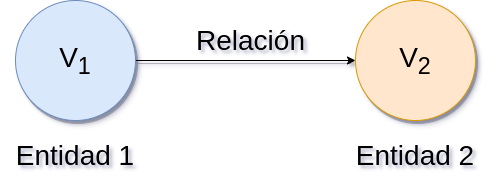
\includegraphics[width=0.40\textwidth]{previo/diagrama.png}
    \caption{Los nodos de los grafos pueden representar recursos o herramientas, personas o instituciones e incluso unidades temáticas. Asimismo, las relaciones entre nodos también llevan asociadas un significado (energía o frecuencia, proximidad o distancia entre ambos o predecedencia u orden entre ambos).}
    \label{fig:classification}
\end{figure}

Los trabajos anteriormente citados así como los que se realizarán en este trabajo fin de grado relacionados con la Minería de Procesos son susceptibles a ser clasificados. Así pues, dado un grafo $G = (V,E)$ donde $V$ y $E$ son sus respectivos conjuntos de vértices y aristas (Definición \ref{def:grafo}) siendo una parte del mismo la que se muestra en la Figura \ref{fig:classification}, se puede realizar una segmentación de los proyectos de minería de procesos atendiendo a qué representan sus nodos, qué significado tiene la relación entre éstos y el momento temporal al que nos estemos refiriendo. Así pues, atendiendo a todas estas características se ha realizado la clasificación de las técnicas de Minería de Procesos en el ámbito educativo que se muestra en el Cuadro \ref{tab:classification}.

\begin{table}[H]
\centering
\caption{Clasificación de las técnicas de Minería de Procesos aplicadas a la educación. Como podemos ver, pueden estar orientadas al pasado, al presente y al futuro.}
\label{tab:classification}
\begin{tabular}{|>{\centering\arraybackslash}m{2.5cm}|>{\centering\arraybackslash}m{9cm}|}
\hline
\rowcolor{orange!20}
\backslashbox{\footnotesize{\textbf{Nodos}}}{\footnotesize{\textbf{Aristas}}} & \footnotesize{\textbf{Energía} (Conteo)} \\ 
\hline 
\cellcolor{orange!20}\footnotesize{Recursos (vídeos, texto) y \textbf{Herramientas}} &

\begin{tabular}[t]{
    | >{\scriptsize\centering\arraybackslash}m{1cm}
    | >{\scriptsize\centering\arraybackslash}m{4cm}|
  }
  \hline
  \cellcolor{cyan!25}\textbf{Pasado} & Coursera\tablefootnote{Coursera Inc. es un proveedor masivo de cursos abiertos en línea.}. Validación del curso. Uso de recursos (como podrían ser los vídeos). \\
  \hline
  \cellcolor{lime!25}\textbf{Presente} & Patrones de uso. Seguimiento. Capacidad. \\
  \hline
  \cellcolor{pink!50}\textbf{Futuro} & Cuellos de botella (predicción de las necesidades del hardware). Posibles problemas. Recomendaciones. \\
  \hline
  \end{tabular}
  
    \\ 
\hline 
\cellcolor{orange!20}\footnotesize{\textbf{Personas} e \textbf{Instituciones}} &

\begin{tabular}[t]{
    | >{\scriptsize\centering\arraybackslash}m{1cm}
    | >{\scriptsize\centering\arraybackslash}m{4cm}|
  }
  \hline
  \cellcolor{cyan!25}\textbf{Pasado} & Trabajo en grupo bien estructurado. Análisis de los alumnos con mejor/peor rendimiento. \\
  \hline
  \cellcolor{lime!25}\textbf{Presente} & Medidas intragrupos e intergrupos. Redes sociales. Evaluación de los alumnos. \\
  \hline
  \cellcolor{pink!50}\textbf{Futuro} & Liderazgo. Dominancia. Personas influyentes. Predicciones del rendimiento de los alumnos. \\
  \hline
  \end{tabular}

\\ 
\hline 
\cellcolor{orange!20}\footnotesize{\textbf{Temáticas} (unidades temáticas de un curso), \textbf{Productos} o \textbf{bienes}} & 

\begin{tabular}[t]{
    | >{\scriptsize\centering\arraybackslash}m{1cm}
    | >{\scriptsize\centering\arraybackslash}m{4cm}|
  }
  \hline
  \cellcolor{cyan!25}\textbf{Pasado} & Validación del curso. Concienciación del profesorado. \\
  \hline
  \cellcolor{lime!25}\textbf{Presente} & Relaciones intergrupos. Redes sociales. \\
  \hline
  \cellcolor{pink!50}\textbf{Futuro} &  \\
  \hline
  \end{tabular}

\\
\hline 
\end{tabular} 
\end{table}